% !TeX root = Bericht.tex
% !TeX spellcheck = en_US
\section{Experimental setup and procedure}\label{sec:procedure}
The experiments begin with a characterization of the Gaussian beam. Afterward, modes of the laser in a cavity are analyzed. 

\subsection{Beam profiling}
The first step is to determine the width of the waist of the beam emitted by a HeNe laser with a wavelength of \( \lambda = 633 \unit{nm} \). After the laser, a Faraday isolator (FI) is placed, which protects the laser from back reflections.

The beam width is measured at various distances from the laser. In total 11 measurements are taken in steps of \SI{1.5}{cm}, starting closely after the FI. The beam width was measured using a waistmeter, which contatins a photodiode measuring the intensity, and a rotating disc. This rotating disc alternately covers the photodiode so that the width of the beam can be determined if the disc's rotation speed and geometry are known. Since the waistmeter indicates the actual diameter, it must later be halved to obtain the radius of the beam.

After these measurements, a lens with a focal length of $f = 100 \unit{mm}$ is placed after the Faraday isolator. The same procedure is then repeated.

\subsection{Mode matching}
\label{subsec:mode}
In preparation for the experiment, the beam waist of the cavity was determined. This can be done using \autoref{eqn:w0} and $r = L = 150 \unit{mm}$ and we get $w_0 = 122.93 \unit{\micro\m}$. 

The next step is to match the resonator waist to the beam waist of the laser using a suitable lens. In \autoref{lens_simulation} the simulated beam with a lens is shown, which is used to determine the best focal length of the lens we want to use for the following steps. In the simulation, the result for the beam diameter and the divergence angle from the first part of the experiment is used. 

\begin{figure}[H]
	\centering
	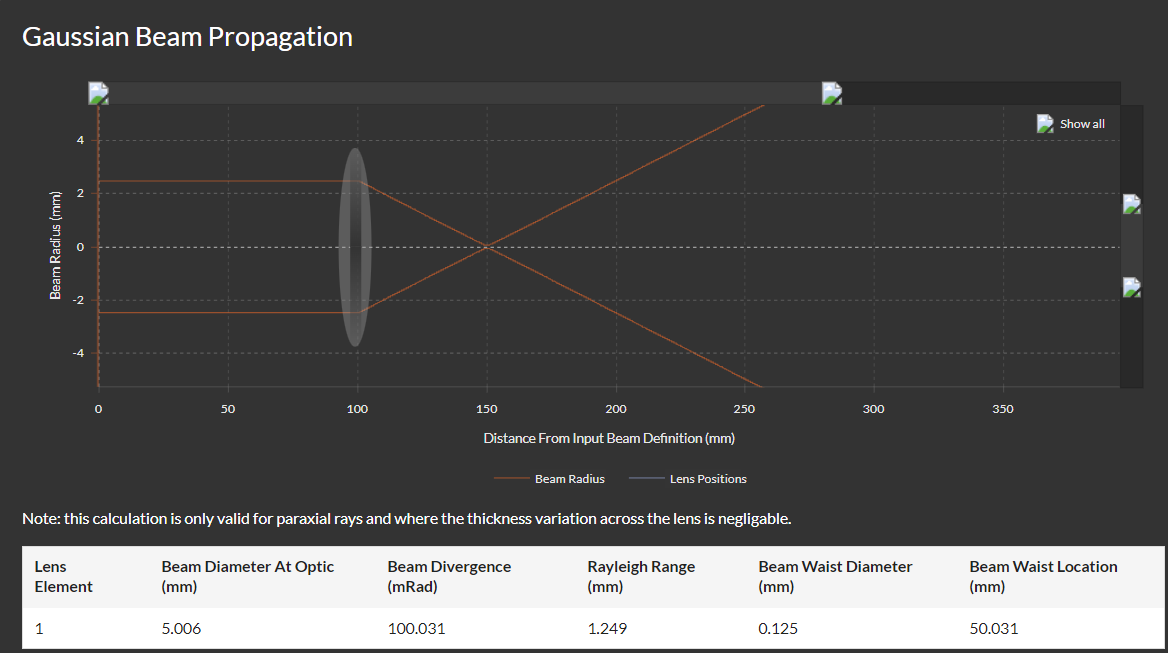
\includegraphics[width=\textwidth]{simulation_lens}
	\caption{Simulation for a Gaussian beam with a beam waist diameter of \SI{0.44}{mm} and a full angle beam divergence of \SI{1.83}{mRad}, including a lens with focal length \SI{200}{mm}, placed at \SI{550}{mm} from the beam focus. Simulation made with \cite{lightmachinery}.} 
	\label{lens_simulation}
\end{figure}

It turns out that \SI{200}{mm} yields the results. Once the lens is in place, the next step is to align it correctly, then adjust the subsequent mirrors and the cavity mirrors to ensure that the laser beam is in a straight line. This entire structure can be seen in \autoref{fig:Gesamtaufbau}. 

\begin{figure}[H]
	\centering
	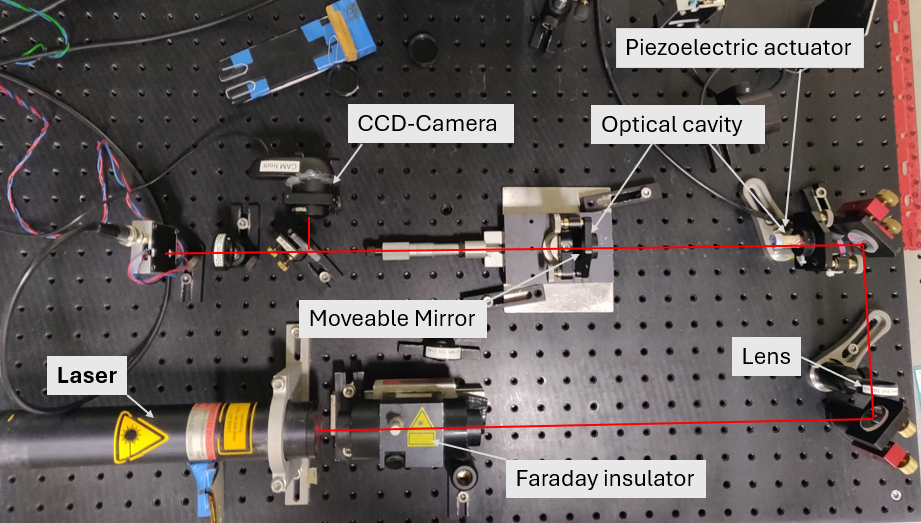
\includegraphics[width=\linewidth]{AufbauBild}
	\caption{The entire setup from the laser to the photodiode and the CCD camera is visible via the Faraday isolator, built-in lens, and optical cavity, which includes a piezoelectric actuator and an adjustable mirror. A beam splitter allows simultaneous irradiation of the two objects. The Faraday isolator ensures that the reflected beam does not return to the laser.}
	\label{fig:Gesamtaufbau}
\end{figure}

After the laser beam leaves the Faraday isolator it passes through a lens and is redirected by two mirrors. It then enters a cavity consisting of two mirrors, one of which is placed on a movable mount, whilst the other is mounted onto a Piezo-transducer, connected to a function generator. This enables us to minimally change the cavities length, effectively scanning frequencies. After the latter cavity mirror, the laser beam passes a beam splitter, directing one part onto a CCD-camera, which is used to take pictures of the incoming beam, while the other part is directed onto a photodiode, connected to an oscilloscope.

\subsection{Study of cavity modes}
\label{subsec:CavityModes}
The resonator is first visually aligned by overlapping the mirror reflections and then fine tuned using the output on the oscilloscope maximizing the transmission of the TEM$_{00}$ mode. Here we recorded two spectra, one with perfect alignment to study the transmission and the other one with slightly misaligned mirrors to measure the distance to half axial modes.

After this, the length of the resonator was increased by \( 13.53(1) \unit{mm} \) using the adjustable mirror to make higher modes visible. In a confocal resonator, these are always projected between two intensity peaks (see \autoref{subsec:OptRes}). One of the deflection mirrors was then adjusted so that the laser no longer falls directly into the resonator. This allows higher modes to be detected on the photodiode, as well as the CCD camera. It is important to note that any change in resonator or laser alignment can affect the visible modes, so careful calibration and control is required throughout the process. The oscilloscope readings and images from the CCD camera are stored for later analysis.
